% kate: word-wrap true;

\chapter{Writing System}

In the past chapter, example words were given in Ayeri's script, \rayr{thno 
hikmu}{Tahano Hikamu}, wherever possible. Thus, it seems advisable to include a 
description of Ayeri's native writing system here as well. Literally, 
\rayr{thno hikmu}{Tahano Hikamu} means `Round Script' (script round), which is 
an old formation based on the word \xayr{thnF/}{tahan-}{write} that  stuck. The 
current word for `script' is \xayr{thnnF}{tahanan}{writing}. Tahano Hikamu was 
originally named thus because of an earlier draft for a script that never made 
it very far beyond the drawing board and which was a lot more angular, or 
\rayr{hinY}{hinya}, see \autoref{fig:hinya}.

\begin{figure}[tp]
\caption{Tahano Hinya and Hikamu}

\begin{minipage}{.5\linewidth}
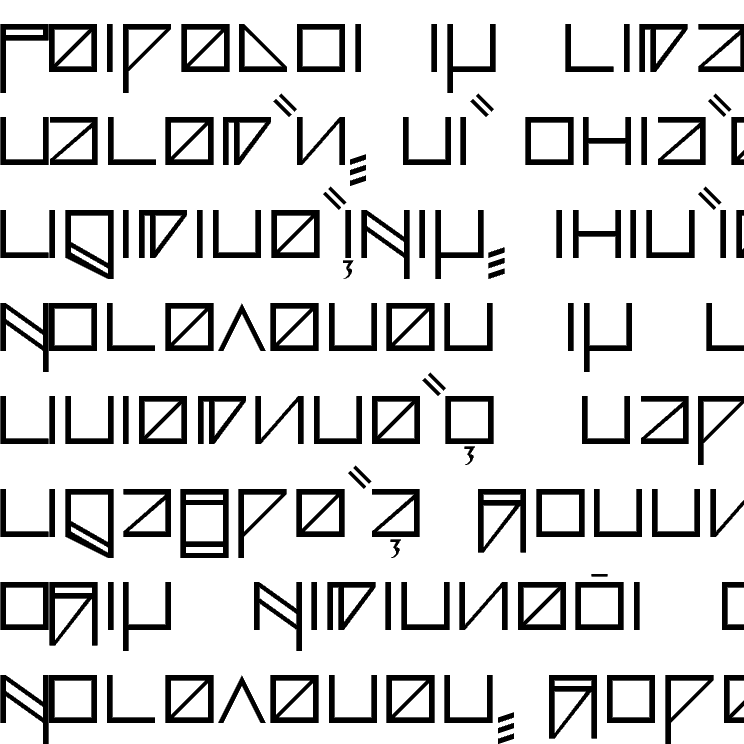
\includegraphics[width=\linewidth]{images/hinya-300dpi-clip.png}
\subcaption{Old and aborted draft: Tahano Hinya}
\label{fig:hinya}
\end{minipage}
~
\begin{minipage}{.5\linewidth}
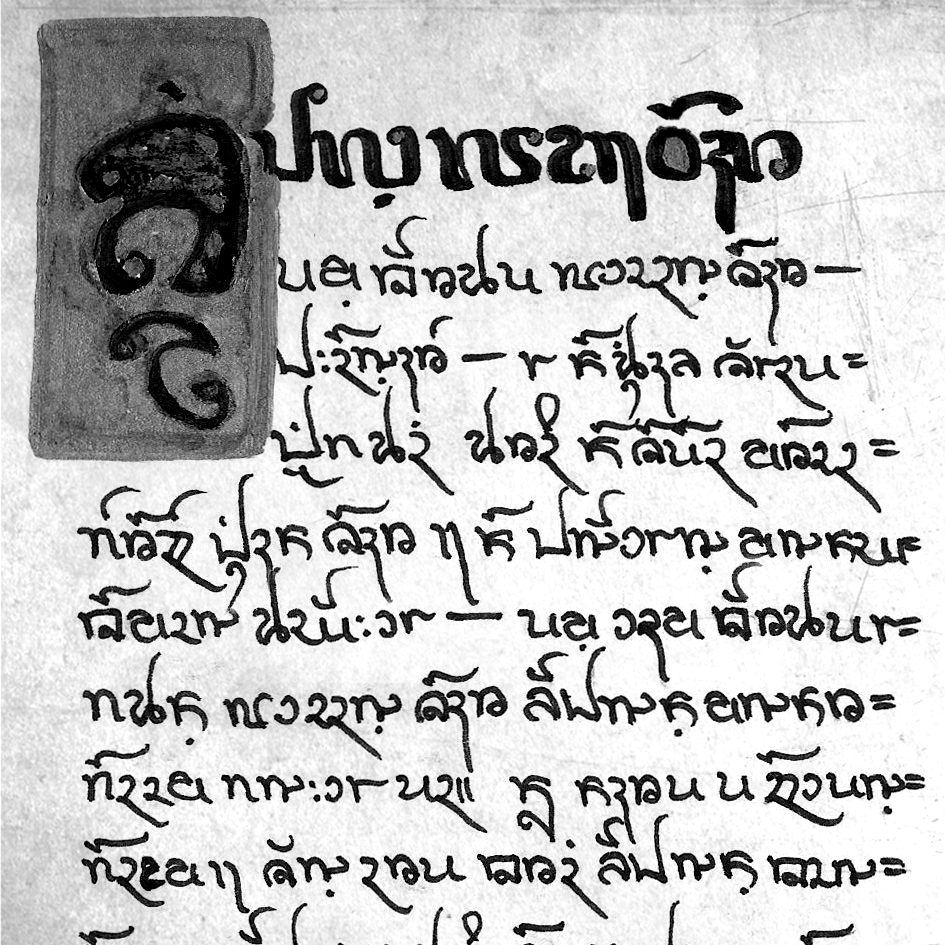
\includegraphics[width=\linewidth]{images/tahano-300dpi-bw-clip.png}
\subcaption{Ayeri's native script: Tahano Hikamu}
\end{minipage}

\label{fig:hinyahikamu}
\end{figure}

As we have seen in the previous chapter, Ayeri's prosody strongly emphasizes 
the syllable as a unit. Thus, it is not a surprise that Ayeri's native script,
Tahano Hikamu, is an alphasyllabary like the Brāhmī-derived alphabets of India 
and Southeast Asia \parencites{salomon1996}{court1996}. This means that its 

\blockcquote[376]{salomon1996}{system is based on the unit of the graphic 
\enquote{syllalbe} […], which by definition always ends with a vowel (type V, 
CV, CCV, etc.). Syllables consisting of a vowel only (usually at the beginning 
of a word or sentence) are written with the \emph{full} or \emph{initial vowel 
signs} […]. But when, as is much more frequently the case, the syllable consists 
of a consonant followed by a vowel, the vowel is indicated by a diacritic sign 
attached to the basic sign for the consonant […].}

Different than in Brāhmī-type scripts, however, Tahano Hikamu does not know 
consonant conjuncts like Devanāgarī {\FS क्ष} \orth{kṣa} ← {\FS क} 
\orth{ka} + {\FS ष} \orth{ṣa}. Another difference from Brāhmī-style scripts is 
that all basic vowels have unique graphemes; vowel length and diphthongs in [ɪ] 
are indicated by dedicated diacritics. Tahano Hikamu also does not know 
subscript notation for consonant clusters and special diacritics marking coda 
consonants like in Javanese \citep[478--479]{kuipersmcdermott1996}. This does 
not mean, however, that final consonants are simply omitted in writing, since 
closed syllalbes are reasonably common enough to warrant indicating them. Thus, 
like in the Sumatran scripts, there is 
\textcquote[476]{kuipersmcdermott1996}{a special mark to eliminate the vowel of 
the previous syllable, thereby leaving a consonant in a syllable-final 
position.} Like in Kharoṣṭhī---another historically important ancient script 
of India---, initial vowels are not represented by unique graphemes but they 
are all written like post-consonantal diacritics with the grapheme for initial 
\fw{a} as a basis, \ayr{A} \citep[377]{salomon1996}. The \ayr{*a} on \ayr{ʔ} is 
understood as a diacritic as well, however, namely for /a/. Similar to the 
Javanese script, Tahano Hikamu puts diacritics not only below or above consonant 
bases, but also before them. This, however, is not limited to vowel graphemes as 
in Javanese \citep[478]{kuipersmcdermott1996}.

\section{Consonants}

Tahano Hikamu is mainly based on consonant bases that are modified by 
diacritics. Since the vowel /a/ is so highly frequent in Ayeri, it is also the 
vowel that is \fw{inherent} to every consonant grapheme if not further modified 
by vowel diacritics. Consonant graphemes are simply referred to as \textit{pa, 
ta, ka, ...} \autoref{fig:consonants} displays all the main graphemes. The 
customary collation is---like the IPA table---grouping the sounds by 
anteriority and sonority.

% \begin{center}\itshape
% 	pa, ta, ka;\\
% 	ba, da, ga;\\
% 	ma, na, nga;\\
% 	va, sa, ha;\\
% 	ra, la, ya;\\
% 	Ø.\\
% \end{center}

\begin{figure}[ht]
\caption{The consonant graphemes of Tahano Hikamu}

\begin{tabu} to \linewidth{X[c] X[c] X[c] X[c] X[c] X[c]}
\toprule
\tableheaderfont	pa & ta & ka & ba & da & ga \\
\rowfont{\Tagati\huge}	p & t & k & b & d & g \\

\midrule

\tableheaderfont	ma & na & ŋa & va & sa & ha \\
\rowfont{\Tagati\huge}	m & n & N & v & s & h \\

\midrule

\tableheaderfont	ra & la & ya & Ø \\
\rowfont{\Tagati\huge}	r & l & y & ʔ \\

\bottomrule
\end{tabu}
\label{fig:thcons}
\end{figure}

